% **************************************************
% Document Class Definition
% **************************************************
\documentclass[%
	paper=A4,					% paper size --> A4 is default in Germany
	twoside=true,				% onesite or twoside printing
	openright,					% doublepage cleaning ends up right side
	parskip=full,				% spacing value / method for paragraphs
	chapterprefix=true,			% prefix for chapter marks
	12pt,						% font size
	headings=normal,			% size of headings
	bibliography=totoc,			% include bib in toc
	listof=totoc,				% include listof entries in toc
	titlepage=on,				% own page for each title page
	captions=tableabove,		% display table captions above the float env
	draft=false,				% value for draft version
]{scrreprt}%

% **************************************************
% Debug LaTeX Information
% **************************************************
%\listfiles

% **************************************************
% Information and Commands for Reuse
% **************************************************
\newcommand{\thesisTitle}{Evolution Analysis of Ethereum Transactions}
\newcommand{\thesisName}{LAM Chi Kong}
\newcommand{\thesisSubject}{COMP5940 Dissertation}
\newcommand{\thesisDate}{December 2020}
\newcommand{\thesisVersion}{0.1}

\newcommand{\thesisFirstReviewer}{First Reviewer}
\newcommand{\thesisFirstReviewerUniversity}{\protect{The Hong Kong Polytechnic University}}
\newcommand{\thesisFirstReviewerDepartment}{Department of Computing}

\newcommand{\thesisSecondReviewer}{Second Reviewer}
\newcommand{\thesisSecondReviewerUniversity}{\protect{The Hong Kong Polytechnic University}}
\newcommand{\thesisSecondReviewerDepartment}{Department of Computing}

\newcommand{\thesisFirstSupervisor}{Dr LUO Xiapu}

\newcommand{\thesisUniversity}{\protect{The Hong Kong Polytechnic University}}
\newcommand{\thesisUniversityDepartment}{Department of Computing}
\newcommand{\thesisUniversityInstitute}{Thesis Research Centre}
\newcommand{\thesisUniversityCity}{Hong Kong}
\newcommand{\thesisUniversityStreetAddress}{Hung Hom, Kowloon}


% **************************************************
% Load and Configure Packages
% **************************************************
\usepackage[utf8]{inputenc}		% defines file's character encoding
\usepackage[english]{babel} % babel system, adjust the language of the content
\usepackage[					% clean thesis style
	figuresep=colon,%
	sansserif=false,%
	hangfigurecaption=false,%
	hangsection=true,%
	hangsubsection=true,%
	colorize=full,%
	colortheme=bluemagenta,%
]{cleanthesis}

\hypersetup{					% setup the hyperref-package options
	pdftitle={\thesisTitle},	% 	- title (PDF meta)
	pdfsubject={\thesisSubject},% 	- subject (PDF meta)
	pdfauthor={\thesisName},	% 	- author (PDF meta)
	plainpages=false,			% 	-
	colorlinks=false,			% 	- colorize links?
	pdfborder={0 0 0},			% 	-
	breaklinks=true,			% 	- allow line break inside links
	bookmarksnumbered=true,		%
	bookmarksopen=true			%
}

\usepackage{booktabs}
\usepackage{amsmath}
\usepackage{multirow,makecell}
\usepackage{url}
\def\UrlBreaks{\do\A\do\B\do\C\do\D\do\E\do\F\do\G\do\H\do\I\do\J
\do\K\do\L\do\M\do\N\do\O\do\P\do\Q\do\R\do\S\do\T\do\U\do\V
\do\W\do\X\do\Y\do\Z\do\[\do\\\do\]\do\^\do\_\do\`\do\a\do\b
\do\c\do\d\do\e\do\f\do\g\do\h\do\i\do\j\do\k\do\l\do\m\do\n
\do\o\do\p\do\q\do\r\do\s\do\t\do\u\do\v\do\w\do\x\do\y\do\z
\do\.\do\@\do\\\do\/\do\!\do\_\do\|\do\;\do\>\do\]\do\)\do\,
\do\?\do\'\do+\do\=\do\#} 

% **************************************************
% Document CONTENT
% **************************************************
\begin{document}

% --------------------------
% rename document parts
% --------------------------
%\renewcaptionname{ngerman}{\figurename}{Abb.}
%\renewcaptionname{ngerman}{\tablename}{Tab.}
\renewcaptionname{english}{\figurename}{Fig.}
\renewcaptionname{english}{\tablename}{Table}

% --------------------------
% Front matter
% --------------------------
\pagenumbering{roman}			% roman page numbing (invisible for empty page style)
%\pagestyle{empty}				% no header or footers
%% !TEX root = ../thesis_phd.tex
%
% ------------------------------------  --> cover title page
\begin{titlepage}
	\pdfbookmark[0]{Cover}{Cover}
	\flushright
	\hfill
	\vfill
	{\LARGE\thesisTitle} \par
	\rule[5pt]{\textwidth}{.4pt} \par
	{\Large\thesisName}
	\vfill
	\textit{\large\thesisDate} \\
	Version: \thesisVersion
\end{titlepage}


% ------------------------------------  --> main title page
\begin{titlepage}
	\pdfbookmark[0]{Titlepage}{Titlepage}
	\tgherosfont
	\centering
	
	{\Large \thesisUniversity} \\[4mm]
	
\includegraphics[width=6cm]{gfx/PolyU_Logo_CMKY} \\[2mm]
	\textsf{\thesisUniversityDepartment} \\
	\textsf{\thesisUniversityInstitute} \\
	%\textsf{\thesisUniversityGroup} \\
	
	\vfill
	{\large \thesisSubject} \\[5mm]
	{\LARGE \color{ctcolormain}\textbf{\thesisTitle} \\[10mm]}
	{\Large \thesisName} \\
	
	\vfill
	\begin{minipage}[t]{.27\textwidth}
		\raggedleft
		\textit{1. Reviewer}
	\end{minipage}
	\hspace*{15pt}
	\begin{minipage}[t]{.65\textwidth}
		{\Large \thesisFirstReviewer} \\
	  	{\small \thesisFirstReviewerDepartment} \\[-1mm]
		{\small \thesisFirstReviewerUniversity}
	\end{minipage} \\[5mm]
	\begin{minipage}[t]{.27\textwidth}
		\raggedleft
		\textit{2. Reviewer}
	\end{minipage}
	\hspace*{15pt}
	\begin{minipage}[t]{.65\textwidth}
		{\Large \thesisSecondReviewer} \\
	  	{\small \thesisSecondReviewerDepartment} \\[-1mm]
		{\small \thesisSecondReviewerUniversity}
	\end{minipage} \\[10mm]
	\begin{minipage}[t]{.27\textwidth}
		\raggedleft
		\textit{Supervisor}
	\end{minipage}
	\hspace*{15pt}
	\begin{minipage}[t]{.65\textwidth}
		\thesisFirstSupervisor%\ and \thesisSecondSupervisor
	\end{minipage} \\[10mm]
	
	\thesisDate \\
	
\end{titlepage}


% ------------------------------------  --> lower title back for single page layout
\hfill
\vfill
\small
\textbf{\thesisName} \\
\textit{\thesisTitle} \\
\thesisSubject, \thesisDate \\
Reviewers: \thesisFirstReviewer\ and \thesisSecondReviewer \\
Supervisor: \thesisFirstSupervisor \\[1.5em]
\textbf{\thesisUniversity} \\
\textit{\thesisUniversityInstitute} \\
\thesisUniversityDepartment \\
\thesisUniversityStreetAddress, \thesisUniversityCity
		% INCLUDE: all titlepages
%\cleardoublepage

%\thesistitlepage{Doctor of Philosophy}%{Temporary Binding for Examination Purposes}
\thesistitlepage{Master of Science in Information Technology}%{Temporary Binding for Examination Purposes}
\cleardoublepage


\pagestyle{plain}				% display just page numbers
\declaration
\cleardoublepage

% !TEX root = ../thesis_phd.tex
%
\pdfbookmark[0]{Abstract}{Abstract}
\chapter*{Abstract}
\label{sec:abstract}
\vspace*{-10mm}

% \blindtext
Ethereum is one of the most popular decentralized platforms for executing computer programs, they often refer to smart contracts which provide extensive applications on top of transferring value in Ether. The records of Ethereum transactions have grown into large datasets since the launch of Ethereum in 2015, there are over 9 million transactions occurred by the end of 2019 and each transaction contains multiple attribute values of different data types. It causes difficulty to understand the evolution of Ethereum transactions related to Ether value transfer, smart contract creation and smart contract invocation, this thesis analyzes these activities with descriptive statistics, regression model and static plots for the entire time period. In addition, this thesis develops an application which allows users to select parties and time intervals for dynamic graph visualization of these activities. The significance of this thesis is to provide a macro-view on distribution and correlation for statistics, micro-view By developing an open-source program for large graph visualization and large graph layout, this paper enables easy access to evolution analysis of Ethereum transactions while reserves customizable functionalities for further development.  To understand major activities of Ethereum transactions including money transfer, contract creation and contract call, this paper conducts evolution analysis to gain new observations.		% INCLUDE: the abstracts (english and german)
\cleardoublepage
%
% !TEX root = ../thesis_phd.tex
%
\pdfbookmark[0]{Acknowledgement}{Acknowledgement}
\chapter*{Acknowledgement}
\label{sec:acknowledgement}
\vspace*{-10mm}

% \blindtext
First of all, I would like to thank my supervisor, Dr LUO Xiapu Daniel, for guiding me to complete this thesis under a difficult time. Daniel is knowledgeable and helpful in leading me to choose an interesting topic, then provides me valuable suggestions on learning the most from this research work.

Before starting this thesis, I had no idea about blockchain and I was not an experienced programmer. It was a huge challenge for me to decide a research topic of analyzing transactions on Ethereum blockchain. Daniel is patient enough to clear all my questions and make me comfortable and confident to take the challenge.

Finally, I would like to thank all my friends who have supported me in completing my thesis. With all of your help, I keep improving myself and solve problems more efficiently. % INCLUDE: acknowledgment
\cleardoublepage
%
\setcounter{tocdepth}{2}		% define depth of toc
\tableofcontents				% display table of contents
\cleardoublepage

\listoffigures
\cleardoublepage

\listoftables
\cleardoublepage

% --------------------------
% Body matter
% --------------------------
\pagenumbering{arabic}			% arabic page numbering
\setcounter{page}{1}			% set page counter
\pagestyle{maincontentstyle} 	% fancy header and footer

% !TEX root = ../thesis.tex
%

\chapter{Introduction}
\label{sec:intro}

% \cleanchapterquote{"Mens cujusque is est Quisque" ¨C "Mind Makes the Man"}{Samuel Pepys}{}

% \blindtext
% 1. Introduction.
% (1)background;(2)The problem to be addressed in this thesis; (3) Your approach; (4) Summary of the applications and the experimental results; (5) Summary of the contributions; (6) Organization of the thesis

\section{Background}
\label{sec:intro:background}

% \blindtext
Ethereum is one of the largest blockchains in terms of market capitalization, the cryptocurrency used in Ethereum transactions is called Ether (ETH). Ethereum is a public blockchain and Ether is distributed based on proof-of-work system, it means miners compete for Ether by consuming resources to solve computationally intensive problems \cite{1}. Similar to Bitcoin blockchain, Ethereum blockchain provides a decentralized platform for transactions to be globally accessible, low-cost, transparent, difficult-to-alter. Different from Bitcoin blockchain, Ethereum blockchain focuses on more than direct value transfer, it provides a global virtual machine for running computer programs as known as smart contracts to cater for complex transactions. For example, a popular application of smart contracts is designing financial products as they often involve complex conditions. To reveal the evolution or growth of blockchain transactions, the graph analysis is conducted in many research studies.

One approach of graph analysis is graph analytics. It constructs graphs with transactions as edges and the participating parties as nodes, then it computes analytics or statistics for the attributes of nodes and edges. For example, centrality measures the importance or significance of individual nodes. Spagnuolo et al. \cite{6} created a modular framework namely "BitIodine", it was applied to multiple real-world cases. In a case related to ransomware, it analyzed the change of significance for known ransomware addresses by investigating the payments from victims' addresses. 

Another approach of graph analysis is community detection. It divides nodes into different clusters to minimize the distances for nodes in the same cluster as well as to maximize the distances for nodes not in the same cluster. Nick \cite{7} summarized several heuristic methods that can be used for clustering in forming communities. His approach included the components "Grapher" and "Classifier", "Grapher" was used for graph construction from transaction data and user data while "Classifier" was used for clustering of nodes by adding tag information as attributes. 

% 1. "The student should provide more background information to explain the research problem.

The significance for the emergence of Ethereum blockchain is the potential of creating a new form of transactions in terms of the diversity of participants, types of activities, security of information, efficiency and cost of establishing contracts, time and place of execution, logical and technical capacity for real-world applications. For the diversity of participants, the Ethereum blockchain has decreasing entry barrier and expanding access channels with its development, it attracts participants from individuals and organizations, different countries, different devices. For the types of activities, currently the major applications on Ethereum blockchain are financial applications which traditionally have standardized services and regulatory requirements. These are typical features of a centralized application which is managed by authorized organizations, they have much weaker role in decentralized applications on Ethereum blockchain because the ownership is largely diluted, it is difficult for a single party to take control of the application even if it is the owner. For the security of information, it is difficult to recognize the identity of an address without additional information provided by its owner, also the address is not uniquely and permanently linked to its owner, therefore the privacy of the owner is protected in some extent. Regarding the public transaction information, it is recorded and shared by all Ethereum clients, the change of data needs consent from over half of the Ethereum clients which constitutes high cost of manipulating transaction information. For the efficiency and cost of establishing contracts, smart contracts are computer programs run on Ethereum Virtual Machine supported by global network of computers, and the transaction fee determined by Ether price is market-driven. For the time and place of transaction execution, currently the Ethereum platform is open all the time and accessible all over the world, it has low geographical restrictions and time cost to establish transactions among different parties. For the logical and technical capacity of real-world applications, the number and diversity of applications built on top the basic utility of moeney transfer continue to growth, some examples include the financial applications, games, social media, productivity software and so on.

To understand the behavioral patterns of Ethereum transactions, this paper raises the following research questions for investigation:
1. How do Ehtereum transactions react to abnormal changes caused by market events?
2. How does the distribution of Ethereum transactions change over time?
3. How do the importance and relationship with neighbors change over time for a specific account?

Based on evolution analysis of Ethereum transactions, this paper obtains the observations below:
1. There was abnormal change in activities of Ethereum transactions in 2018, a relevant significant event was the launch of a stable cryptocurrency Dai.
2. The decentralized exchange, "Allbit" had the most contract invocation transactions associated among all studied decentralized exchanges in 2018, it introduced the cryptocurrency Dai into its products.
3. In 2018, "Allbit" beated its predecessor "DEx.top" in terms of centrality and community measures of contract invocation.

\section{Proposed Approach}
\label{sec:intro:proposed}

% \blindtext
This thesis proposes a approach considering the macro view and micro view of Ethereum transactions, which serves for the applications such as abnormality detection, impact analysis, evolutionary study.

From the macro view, the growth of smart contracts is analyzed by descriptive statistics and visualized by time plots. It can be applied to abnormality detection to inspect unusual changes in descriptive statistics, which can indicate significant events. In section \ref{sec:evaluation:abnormality}, it was found that in 2018 the activities of contract creation and decreation have abnormal changes, and the issuance of stable currency Dai was a significant event in that year.

From the micro view, a program is developed to visualize three major transaction activities including money transfer, smart contract creation and smart contract invocation. It can be applied to impact analysis to visualize the distribution of transaction activities on individual accounts. In section \ref{sec:evaluation:impact}, it was found that in 2018 the sharp increase in contract invocation was contributed mostly by the decentralized exchange "Allbit". Moreover, it can be applied to evolutionary study to illustrate the change in importance of individual accounts and their relationships with others. In section \ref{sec:evaluation:evolution}, it was found that in 2018 the "Allbit" grew sharply in contract invocation and exceeded another decentralized exchange "DEx.top".

This thesis makes the following contributions. From the macro view, transactions over the entire study period are fully imported without down sampling, they are grouped by day to reduce computational complexity, this approach can preserve the population data and extract relevant details. From the micro view, it enables user interaction to select specific accounts and time intervals for dynamic graph generation. Also, it is open-source to non-developers for direct execution and for developers for further customization. To the best of our knowledge, this thesis is the first research paper proposing a approach on fulfilling all of above requirements.

\section{Thesis Structure}
\label{sec:intro:structure}

The remaining chapters of this thesis are organized as below.

\textbf{Chapter \ref{sec:review}: Related Work} \\[0.2em]
% \blindtext
This chapter includes sections Ethereum Transactions, Evolution Analysis, New Perspective.

\textbf{Chapter \ref{sec:methodology}: Methodology} \\[0.2em]
% \blindtext
This chapter includes sections Data Collection, Statistical Analysis, Graph Visualization. Data Collection includes subsections Statistical Data and Graph Data. Statistical Analysis includes subsections Descriptive Statistics and Regression Model. Graph Visualization includes subsections Data View, Graph View, Node View, Control View.

\textbf{Chapter \ref{sec:applications}: Applications} \\[0.2em]
% \blindtext
This chapter includes sections Abnormality Detection, Impact Analysis, Evolutionary Study.

\textbf{Chapter \ref{sec:evaluation}: Evaluation} \\[0.2em]
% \blindtext
This chapter includes sections Abnormality Detection, Impact Analysis, Evolutionary Study. Abnormality includes subsections Creation Statistics, Decreation Statistics, Significant Event. 

\textbf{Chapter \ref{sec:conclusion}: Conclusion} \\[0.2em]
% \blindtext
This chapter includes sections Major Contributions and Future Improvements.
 % INCLUDE: introduction
% !TEX root = ../thesis.tex
%
\chapter{Related Work}
\label{sec:review}

% \cleanchapterquote{"Mens cujusque is est Quisque" ¨C "Mind Makes the Man"}{Samuel Pepys}{}

% \blindtext
% 2. Related work
% (1) Blockchain, in particular Ethereum; (2) Transaction analysis; (3) Visualization for Blockchain; (4) Difference between your work and existing studies.

\section{Ethereum Transactions}
\label{sec:review:transactions}

% \blindtext
In the simplest terms, blockchain represents an unchangeable digital ledger system. A distinctive feature of blockchain technology is its distributed implementation, further discussions on blockchain can be found in many publications \cite{9}. Bitcoin blockchain is one of the best known blockchains for speculation in Bitcoin cryptocurrency and payments with Bitcoin wallets. Ethereum blockchain is another popular blockchain for executing complex transactions on top of transferring value in its cryptocurrency Ether. It allows to create smart contracts and enables users to create crypto-assets. For example, Ethereum tokens are sold in the event of Initial Coin Offering (ICO) \cite{10}. Such token ICOs have attracted many startups and organizations to raise funds by selling digital coins that allow recipients to use the promised service as much as possible. In the years of 2018 and 2019, Ethereum ICO raised billions of dollars. While fluctuations in Ether prices are not Ethereum transactions, ICO is a process involving many Ehtereum transactions.

\begin{figure}[htb]
	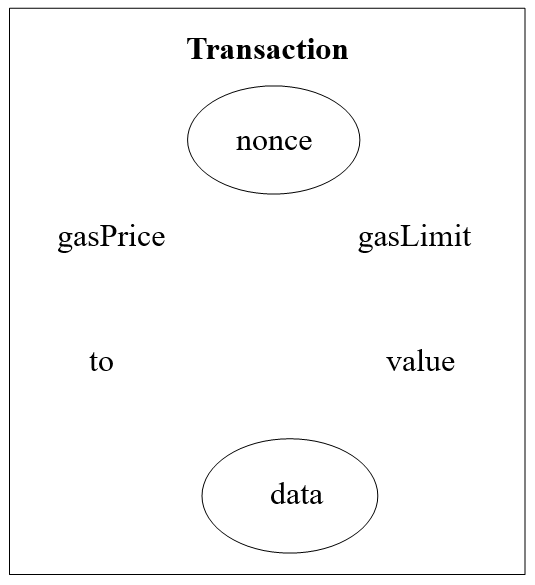
\includegraphics[width=0.7\textwidth]{gfx/transactions.png}
	\caption{Example of an External Transaction}
	\label{fig:transactions}
\end{figure}

Ethereum is a state machine based on transactions. In other words, a transaction occurred between two different accounts converts Ethereum globally from one state to another \cite{13}. A transaction is executed in a block, its two accounts are the source and target. These accounts can be Externally Owned Accounts (EOAs) or smart contracts, EOAs are serialized and then submitted to the blockchain. There are two types of transactions including external transactions and internal transactions. In an external transaction, the sender (source) account is an EOA, the recipient (target) account is an EOA if the transaction is money transfer or it is a contract account if the transaction is contract creation or contract invocation \cite{14}. The data fields of an external transaction include account addresses, timestamp, value and others \cite{16}. The Fig. \ref{fig:transactions} shows typical elements of an external transactions. For an internal transaction, the source account is smart contract instead of EOA, its corresponding activities are transferring money to EOA, creating smart contract and invoking smart contract which are the same for an external transaction. Every account has a nonce keeping track of the transactions they perform, it can be used to prevent replay attacks. A transaction is a list of operations to be executed, gas for an operation is relatively fixed and required to perform this operation. The gasPrice field represents the price per unit of gas you are willing to pay while the gasLimit field determines how many units of gas you are willing to pay for.

\section{Evolution Analysis}
\label{sec:review:evolution}

% \blindtext
Regarding transaction analysis, Chen et al. analyze all the Ethereum transactions from 30 Jul 2015 to 10 Jun 2017 by constructing Money Flow Graph (MFG) for money transfer, Contract Creation Graph (CCG) for smart contract creation and Contract Invocation Graph (CIG) for smart contract invocation \cite{3}. They also provide graph analytics as measures of degree, clustering, correlation, importance, assortativity and connected components. Yue et al. develop a web application called BitExTract for interactive visualization of Bitcoin exchanges, it provides views including exchanges list panel for selecting exchanges, massive sequence view for related news, connection view for inter-exchange relationships grouped by geographical region and comparison view for transaction amounts over time \cite{19}. It is worth noting that it enables users to select exchanges and time interval, which gives users flexibility to extract information about evolution of Bitcoin exchanges.

Regarding graph visualization, Lanum suggests Gephi which is a Graphical User Interface (GUI) written in Java for building graph visualization, it provides many options for configuring its built-in UI \cite{4}. Meanwhile, there is a considerable learning cost of these Gephi-specific configurations, and the manual process of data handling is not as ideal as automated scripts for large datasets. Meeks recommends D3.js which is a JavaScript library for web-based interactive visualization to visualize graph data, it enables data filtering, graph construction and graph visualization all in scripts \cite{5}. There is also a learning cost of configuring graph visualization in JavaScript, and more importantly an efficient algorithm and data representation are required to process and visualize large scale of graph data given the limited capacity of browser.

\section{New Perspective}
\label{sec:review:perspective}

Despite the popularity of Ethereum blockchain, there is a lack of in-depth analysis on the evolution of Ethereum transactions. This thesis proposes the macro view and micro view to visualize Ethereum transactions. With the focus on evolution analysis, the macro view covers all the Ethereum transactions from 30 Jul 2015 to 25 Nov 2019 without sampling, and groups the transactions by day instead of the entire period. Moreover, the micro view is provided by an application developed in this thesis for graph visualization over time, this application allows users to interact with graphs for selected accounts and time intervals, it is open-source to developers and non-developers for direct implementation or further customization. To the best of our knowledge, this thesis is the first research work proposing the evolution analysis of Ethereum transactions satisfying all of the above criteria.

For the macro view, there are different metrics in daily transactions for activities related to smart contract as an important feature of Ethereum blockchain. These activities include contract creation which is positive for the growth of smart contracts, and contract decreation which is negative for the growth of smart contracts. To understand the evolution of contract activities, this thesis computes the descriptive statistics of the metrics and visualizes them with time plots. Besides, this thesis constructs a regression model to investigate contract suicide and its correlated factors.

For the micro view, this thesis develops an application to visualize node relationships and interact with graphs on top of constructing MFG, CCG and CIG based on the existing work. To visualize node relationships, the application can highlight the neighbors of a specific node and their edges to observe their relationships, it introduces community measures of Louvain community, label propagation community and union find community upon centrality measures to illustrate relationships among groups of nodes. To interact with graphs, the application provides flexibility for users to select accounts, time intervals and value ranges to generate graphs dynamically.

\section{Research Significance}
\label{sec:review:significance}
% 2.  Moreover, the student should clearly explain the differences between this work and other studies

% 3. and highlight the contributions of this dissertation

The existing approaches of analyzing Ethereum transactions are mainly based on static analysis or static data. The static analysis usually has fixed configuration and parameters, and is not publicly available as the open-source projects. The static data is usually the processed form, and the program to collect and transform the data is missing, therefore the data cannot be retrieved upon user requests and stays updated. These problems lead to the lack of flexibility to reuse and customize the analytical model. 

The model is not reusable when it cannot be applied to different datasets to verify its validity and accuracy. The programs for this type of models usually have restrictions on the choices of analysis, variability of time period and interaction with users. For the case in analyzing Ethereum transactions, many research studies adopt fixed time period and provide cumulative statistics, where the behavioral patterns of Ethereum transactions over time are omitted. Some of them are not open-source or provide solely the static analysis result that does not allow user interaction during data visuaization, the users cannot reuse the model for other applications, or even cannot reproduce the analytical results published by the research papers.

The model specifically designed for the investigated dataset usually lacks the capacity for customization. If the data model can only process a predefined dataset, then it has little value for users to study the model. For the case of graph visualization of Ethereum transactions, Users may want the customization on the selection of nodes (e.g. different types of exchange addresses), start date and end date, type of activity (money transfer, contract creation, contract invocation), graph analytics (centrality, community), information of neighbor nodes, selection of time range to illustrate the evolution of Ethereum transactions.

With regard to the above problems, this paper develops a program for interactive graph visualization of Ethereum transactions with the following contributions:
1. Developing a reusable program to visualize graph datasets
2. Developing an open-source program which can be customized to enhance interactive graph visualization
3. Provide use cases of this prgram including the abnormality detection, impact analysis, evolutionary study explained in details at Section \ref{sec:applications}. % INCLUDE: related work
% !TEX root = ../thesis.tex
%
\chapter{Methodology}
\label{sec:methodology}

% \cleanchapterquote{Innovation distinguishes between a leader and a follower.}{Steve Jobs}{(CEO Apple Inc.)}

\section{Data Collection}
\label{sec:methodology:data}

% \begin{figure}[htb]
% 	
\includegraphics[width=\textwidth]{gfx/Clean-Thesis-Figure}
% 	\caption{Figure example: \textit{(a)} example part one, \textit{(c)} example part two; \textit{(c)} example part three}
% 	\label{fig:system:example1}
% \end{figure}

% \blindtext

% \blindtext

% \begin{figure}[htb]
% 	
\includegraphics[width=\textwidth]{gfx/Clean-Thesis-Figure}
% 	\caption{Another Figure example: \textit{(a)} example part one, \textit{(c)} example part two; \textit{(c)} example part three}
% 	\label{fig:system:example2}
% \end{figure}

% \blindtext
% 3. Methodology
% (1) Purposes; (2) Challenges; (3) Your methodology (including data collection, data analysis, data visualization, etc.); (4) Implementation

\begin{figure}[htb]
	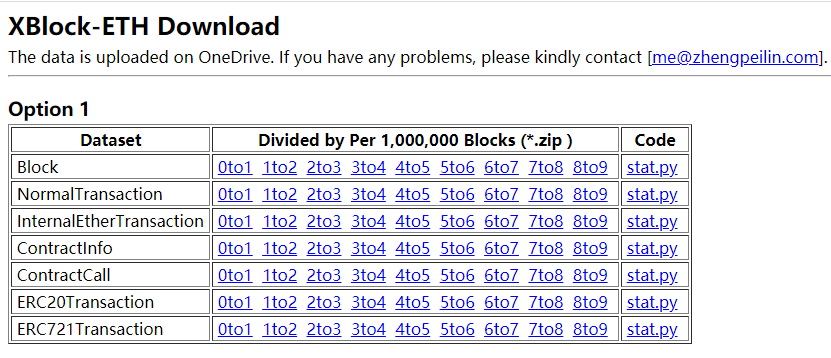
\includegraphics[width=\textwidth]{gfx/data.png}
	\caption{Datasets of Ethereum Transactions}
	\label{fig:data}
\end{figure}

Google BigQuery provides a public dataset which contains updated information of Ethereum transactions. However, it adds complexity in configuring Google account to retrieve data greater than 1 GB, and data size in this thesis is above 100 GB. As an alternative, this thesis adopts data that comes from Xblock website \cite{21}. The datasets of Ethereum transactions are shown in Fig. \ref{fig:data}.

For dataset "Block", it records information related to blocks and its data fields include "blockNumber", "timestamp", "gasUsed", "miner", "reward" and others. For dataset "NormalTransaction", it records information related to external transactions and its data fields include "blockNumber", "timestamp", "from", "to", "creates", "value" and others. For dataset "InternalEtherTransaction", it records information related to internal transactions and its data fields include "blockNumber", "timestamp", "from", "to", "fromIsContract", "toIsContract", "value" and others. For dataset "ContractInfo", it records information related to contract creation and decreation and its data fields include "address", "createdTimestamp", "creator", "decreatedTimestamp", "refunder", "refundValue" and others. When a smart contract is decreated (or deleted), it costs gas to compensate miners for executing this transaction, then some refund value is sent from the refunder to specific accounts. For dataset "ContractCall", it records information related to contract invocation (or call) and its data fields include "blockNumber", "timestamp", "from", "to", "fromIsContract", "toIsContract", "value" and others. When a smart contract is called, it is executed to perform operations defined in contract code. For dataset "ERC20Transaction", it records information related to ERC20 tokens and its data fields include "blockNumber", "timestamp", "tokenAddress", "from", "to", "value" and others. For dataset "ERC721Transaction", it records information related to ERC721 tokens and its data fields include "blockNumber", "timestamp", "tokenAddress", "from", "to", "tokenId" and others. ERC20 and ERC721 are two design standards for Ethereum tokens, they facilitate the development of smart contracts for token issuance and comparison among different tokens. Tokens are frequently used for fundraising and play a similar role as shares of listed companies.

These datasets cover the Ethereum transactions from block 0 on 30 Jul 2015 to block 8,999,999 on 25 Nov 2019. The dataset "ContractInfo" forms the statistical data to compute descriptive statistics and to formulate regression model for investigating the growth of contract activities. Datasets "NormalTransaction", "InternalEtherTransaction", "ContractInfo" and "ContractCall" form the graph data to construct MFG, CCG and CIG for graph visualization of evolving transaction activities.

\subsection{Statistical Data}
\label{sec:methodology:data:statistical}

\begin{figure}[htb]
	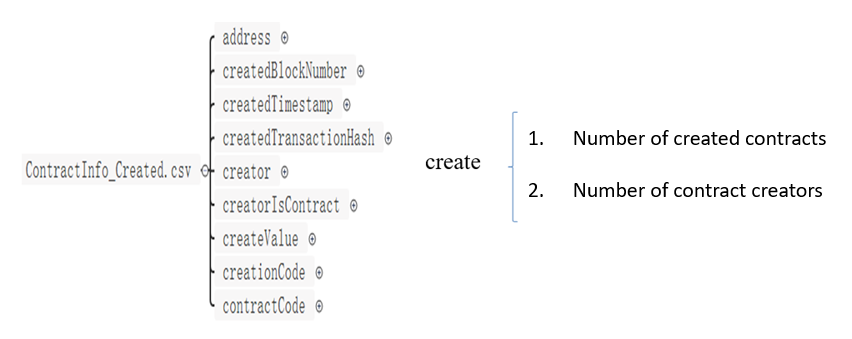
\includegraphics[width=0.95\textwidth]{gfx/statistical1.png}
	\caption{Data fields for contract creation}
	\label{fig:statistical1}
\end{figure}

\begin{figure}[htb]
	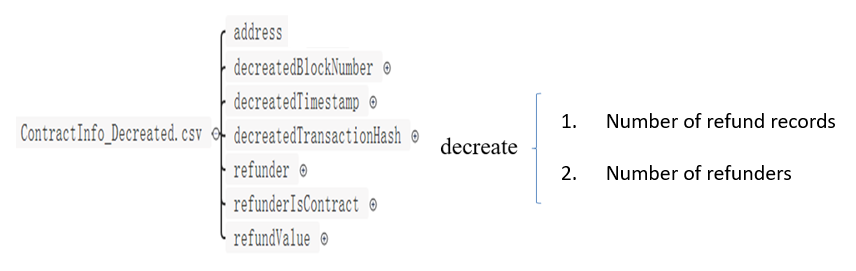
\includegraphics[width=\textwidth]{gfx/statistical2.png}
	\caption{Data fields for contract decreation}
	\label{fig:statistical2}
\end{figure}

The dataset "ContractInfo" consists of transaction information related to smart contract creation and decreation.

Transactions for smart contract creation are recorded with data fields shown in Fig. \ref{fig:statistical1}, these transactions are grouped by day to compute the metrics including daily number of created contracts and daily number of contract creators. Then, the metrics are used to compute descriptive statistics and to draw time plots.

Transactions for smart contract decreation are recorded with data fields shown in Fig. \ref{fig:statistical2}, these transactions are grouped by day to compute the metrics including daily number of refund records and daily number of refunders. Then, the metrics are used to compute descriptive statistics and to draw time plots. They are also used to formulate a regression model that describes the correlated factors of refund.

\subsection{Graph Data}
\label{sec:methodology:data:graph}

The relevant datasets are processed in the following order:

1. The dataset "ContractInfo" is used to obtain all "ccg\_nodes" and "ccg\_edges" of CCG data. For "ccg\_nodes", its "node\_name" and "node\_type" are determined by "address" in "ContractInfo". For "ccg\_edges", its "from\_name", "to\_name", "time\_stamp" are determined by "creator", "address", "createdTimestamp" in "ContractInfo".

2. The dataset "ContractCall" is used to obtain all "cig\_nodes" and "cig\_edges" of CIG data. For "cig\_nodes", its "node\_name" and "node\_type" are determined by "from", "fromIsContract", "to", "toIsContract" in "ContractCall". For "cig\_edges", its "from\_name", "to\_name", "time\_stamp", "number\_of\_calls" are determined by "from", "to", "timestamp" in "ContractCall".

3. The dataset "InternalEtherTransaction" is used to obtain partial "mfg\_nodes" and "mfg\_edges" of MFG data. For "mfg\_nodes", its "node\_name" and "node\_type" are determined by "from", "fromIsContract", "to", "toIsContract" in "InternalEtherTransaction". For "mfg\_edges", its "from\_name", "to\_name", "time\_stamp", "value\_in\_ether" are determined by "from", "to", "timestamp", "value" in "InternalEtherTransaction".

4. The dataset "NormalTransaction" is used to obtain remaining "mfg\_nodes" and "mfg\_edges" of MFG data. For "mfg\_nodes", its "node\_name" and "node\_type" are determined by "from", "fromIsContract", "to", "toIsContract" in "NormalTransaction". For "mfg\_edges", its "from\_name", "to\_name", "time\_stamp", "value\_in\_ether" are determined by "from", "to", "timestamp", "value" in "NormalTransaction".

During the extraction of graph data, the addresses of exchanges are converted to their names for identification of exchanges later in graph visualization, the address-name pairs of exchanges are found in exchange directory on EtherScan \cite{17}. Finally, the extracted nodes and edges are stored as collections in a database called "ethereum\_tx".

\section{Statistical Analysis}
\label{sec:methodology:analysis}

\subsection{Descriptive Statistics}
\label{sec:methodology:analysis:statistics}

\begin{table}[h]
\caption{Example of descriptive statistics}
\label{tab:descriptive-statistics}
\renewcommand\arraystretch{0.7}
\begin{tabular}{@{}cc@{}}
\toprule
\multicolumn{2}{c}{Daily number of created contracts} \\
\midrule
Average                & 12267.14442    \\
Standard Error         & 366.8075104    \\
Median                 & 7510.5         \\
Mode                   & 7267           \\
Standard Deviation     & 11089.48345    \\
Variance               & 122976643.2    \\
Kurtosis               & 2.305335977    \\
Skewness               & 1.789698857    \\
Minimum                & 650            \\
Maximum                & 52959          \\
Summation              & 11212170       \\
Observation            & 914            \\
\bottomrule
\end{tabular}
\end{table}

\begin{figure}[htb]
	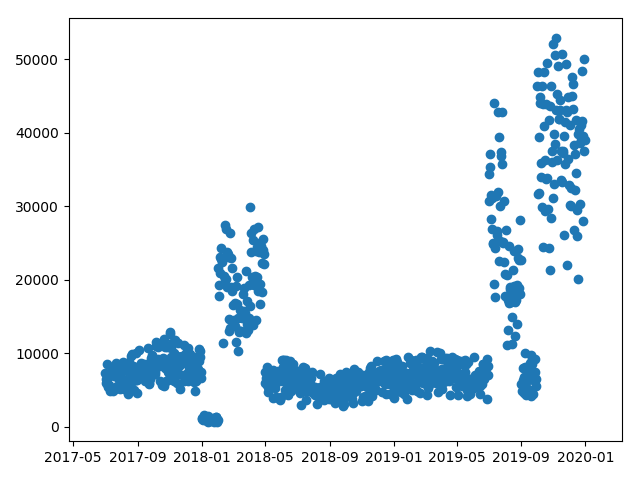
\includegraphics[width=0.7\textwidth]{gfx/created-contracts.png}
	\caption{Example of a time plot}
	\label{fig:created-contracts}
\end{figure}

Statistical data representing contract creation and contract decreation is used to compute descriptive statistics and to draw time plots. An example of descriptive statistics is shown in Table \ref{tab:descriptive-statistics}, these statistics describe the distribution of metric for all observation days with "Average", "Standard Error", "Median", "Mode, "Standard Deviation", "Variance", "Kurtosis", "Skewness", "Minimum", "Maximum", "Summation" and "Observation". Moreover, the change of metric is illustrated by a time plot to visualize its trend, an example is shown in Fig. \ref{fig:created-contracts}.

\subsection{Regression Model}
\label{sec:methodology:analysis:model}

\begin{table}[h]
\caption{Correlation coefficient matrix}
\label{tab:correlation-matrix}
\begin{tabular}{|c|c|c|c|c|c|c|}
\hline
\multicolumn{7}{|c|}{Correlation coefficient matrix} \\
\hline

\multicolumn{2}{|c|}{} &
\makecell{Created\\ Contracts} & \makecell{Contract\\ Creators} & \makecell{Refund\\ Records} & Refunders & \makecell{Refund\\ Amount} \\
\hline

\multirow{2}{*}{
\makecell{Created\\ Contracts}} & Related & 1 & -0.038 & .169** & .253** & -.148** \\
\cline{2-7} & significant & & 0.256 & 0.000 & 0.000 & 0.000 \\
\hline
\multirow{2}{*}{Contract Creators} & Related & -0.038 & 1 & .349** & .153** & -0.017 \\
\cline{2-7} & significant & 0.256 & & 0.000 & 0.000 & 0.605 \\
\hline
\multirow{2}{*}{
\makecell{Refund\\ Records}} & Related & .169** & .349** & 1 & .426** & -0.005 \\
\cline{2-7} & significant & 0.000 & 0.000 & & 0.000 & 0.878 \\
\hline
\multirow{2}{*}{Refunders} & Related & .253** & .153** & .426** & 1 & -.148** \\ 
\cline{2-7} & significant & 0.000 & 0.000 & 0.000 & & 0.000 \\
\hline
\multirow{2}{*}{
\makecell{Refund\\ Amount}} & Related & -.148** & -0.017 & -0.005 & -.148** & 1 \\
\cline{2-7} & significant & 0.000 & 0.605 & 0.878 & 0.000 &  \\[10pt]
\hline
\multicolumn{7}{|l|}{*. At level 0.05, the correlation was significant} \\ 
\hline
\multicolumn{7}{|l|}{**. At level 0.01, the correlation was significant} \\ 
\hline
\end{tabular}
\end{table}

Regarding the daily refund amount, the potentially correlated variables including daily number of created contracts as "Created Contracts", daily number of contract creators as "Contract Creators", daily number of refund records as "Refund Records", daily number of refunders as "Refunders", daily refund amount as "Refund Amount" are investigated with the correlation coefficient matrix in Table \ref{tab:correlation-matrix}. The correlation coefficients in the matrix are Pearson correlation coefficients. In Table \ref{tab:correlation-matrix}, the rows "Related" and "significance" contain the test statistics of correlation coefficients for each pair of variables and their significance under two-tailed hypothesis testing respectively. If the significance is below a level, 0.05 or 0.01, it is said to be statistically significant to conclude that the pair of variables are correlated.

From the results of correlation coefficient matrix, the daily refund amount is statistically correlated to the daily number of created contracts and daily number of refunders both at significance level 0.01. Therefore, the daily number of created contracts and daily number of refunders are fitted to linear regression model to predict the daily refund amount. The regression statistics are shown in Table \ref{tab:regression-statistics}.

\begin{table}[h]
\caption{Regression Statistics}
\label{tab:regression-statistics}
\begin{tabular}{c|c}
\hline
\multicolumn{2}{c}{Regression Statistics} \\
\hline
Multiple R & .839a \\
\hline
R Square & .704 \\
\hline
Adjusted R Square & .653 \\
\hline
Standard Error & 320.299643300000000 \\
\hline
Observations & 914 \\
\hline
\end{tabular}\\
\end{table}

From the regression statistics, the R Square is 70.4\%, it means that 70.4\% of variation in daily refund amount can be explained by the daily number of created contracts and daily number of refunders. In addition, the Analysis Of Variance (ANOVA) is performed to further investigate the relations between these variables, the results are provided in Table \ref{tab:anova-table}.

\begin{table}[h]
\caption{ANOVA Table}
\label{tab:anova-table}
\begin{tabular}{c|c|c|c|c}
\hline
\multicolumn{5}{c}{ANOVA Table} \\
\hline
 & Coefficients & Standard Error & t Stat & P-value \\
\hline
Intercept & 183.198 & 25.191 & 7.273 & .000 \\
\hline
Created Contracts & -0.005 & .001 & -4.953 & .000 \\
\hline
Refunders & .081 & .026 & 3.102 & .002 \\
\hline
\end{tabular}
\end{table}

From ANOVA table, the P-values of intercept, daily number of created contracts and daily number of refunders are all below 0.01, it implies they are statistically significant to be included in the linear regression model. By considering the coefficients of these explanatory variables, the resultant regression model can be written as:

$$\text{Refund Amount} = 183.198 - 0.005 * \text{Created Contracts} + 0.081 * \text{Refunders}$$

\section{Graph Visualization}
\label{sec:methodology:view}

\begin{table}[h]
\caption{Development Challenges}
\label{tab:development-challenges}
\begin{tabular}{@{}cc@{}}
\toprule
Challenge & Module      \\
\midrule
Interactive UI & PyQt5       \\
Large graph visualization & Vispy       \\
Large graph layout & PyGraphviz  \\
Portable program & PyInstaller \\
\bottomrule
\end{tabular}
\end{table}

The major development challenges for graph visualization of Ethereum transactions are listed in Table \ref{tab:development-challenges}, they include interactive User Interface (UI), large graph visualization, large graph layout, portable executable program. These challenges are handled by the following Python modules.

PyQt5 represents UI elements as Python classes, their style can be modified by changing the property values while their behavior can be altered by linking to a function \cite{2}. The built-in Qt designer can be used to create UI elements and convert them into code, then only the functions need to be programmed.

Vispy leverages the computing power of GPU to achieve high performance in large data visualization \cite{12}. It is mainly applied to filtering out the subgraph and computing the graph analytics (i.e. centrality and community measures).

PyGraphviz provides fast algorithms of generating large graph layout which avoids overlapping edges for clear visualization \cite{15}.

PyInstaller is a light-weight packaging manager to convert Python program to executable, in this paper it is used to create portable version of the program \cite{20}.

The program for graph visualization is shown in Fig. \ref{fig:view}. It is composed of four core components, namely data view (Fig. \ref{fig:view}A), graph view (Fig. \ref{fig:view}B), node view (Fig. \ref{fig:view}C) and control view (Fig. \ref{fig:view}D).

\begin{figure}[htb]
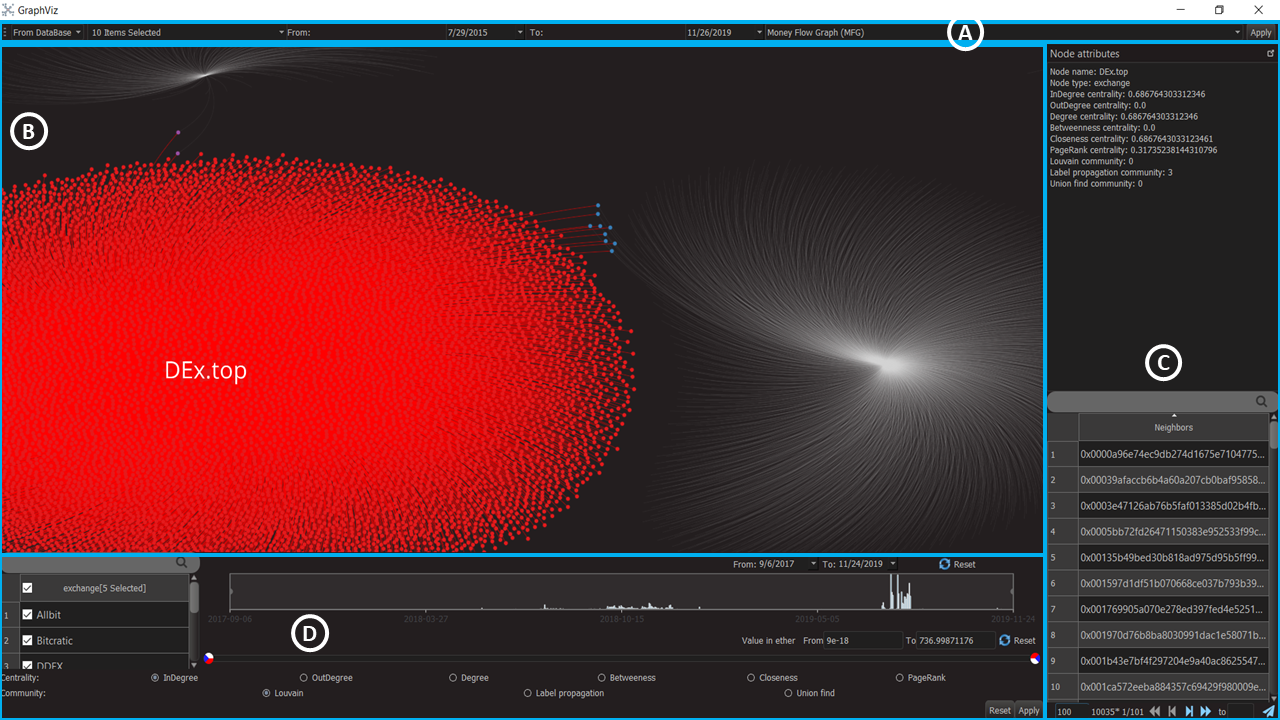
\includegraphics[width=\textwidth]{gfx/view.png}
\caption{Graph visualization is divided into four components including (A) data view, (B) graph view, (C) node view and (D) control view.}
\label{fig:view}
\end{figure}

\subsection{Data View}
\label{sec:methodology:view:data}

\begin{figure}[htb]
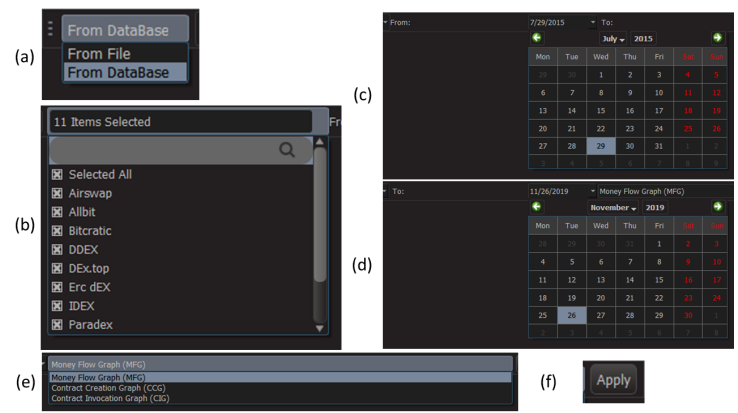
\includegraphics[width=0.7\textwidth]{gfx/data-view.png}
\caption{Data view consists of (a) options to select data source, (b) options to select exchange names, (c) options to select starting date, (d) options to select ending date, (e) options to select graph type and (f) retrieval of data under selection criteria.}
\label{fig:data-view}
\end{figure}

The data view acts as a menu bar for users to specify the selection criteria to retrieve data from the data source. The available options are in the groups of data source (Fig. \ref{fig:data-view}a), exchange names (Fig. \ref{fig:data-view}b), starting date (Fig. \ref{fig:data-view}c), ending date (Fig. \ref{fig:data-view}d) and graph type (Fig. \ref{fig:data-view}e). The "Apply" button (Fig. \ref{fig:data-view}f) combines these selection options to retrieve data for graph construction.

The selection of data source is to retrieve transactions from either a GEXF file or the MongoDB database. GEXF format is the default format in Gephi representing data structure of graph in the form of nodes and edges.

The selection of exchange names is to retrieve transactions where each transaction has its from address or to address in the list of selected exchanges. The exchange names are grouped by exchange type and sorted alphabetically.

The selection of starting date and ending date is to retrieve transactions occurred between these two dates. The default starting date is one day before the first transaction while the default ending date is one day after the last collected transaction.

The selection of graph types is to retrieve transactions based on three major activities, namely MFG for money transfer, CCG for contract creation, CIG for contract invocation.

Moreover, the program supports the opening of multiple windows which facilitates the comparison analysis. For examples, transactions for the same exchanges in different time periods can be compared in different windows, or transactions for different categories such as crypto exchanges and decentralized exchanges can be compared in different windows.

\subsection{Graph View}
\label{sec:methodology:view:graph}

\begin{figure}[htb]
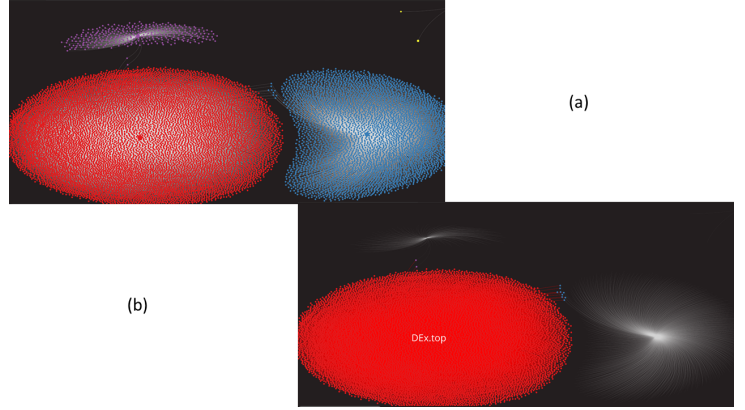
\includegraphics[width=0.7\textwidth]{gfx/graph-view.png}
\caption{Graph view shows the effects of nodes and edges (a) before clicking a node and (b) after clicking a node.}
\label{fig:graph-view}
\end{figure}

The graph view is used to display the nodes and edges after graph construction. Before clicking a node (Fig. \ref{fig:graph-view}a), nodes of different sizes and colors are connected by light gray edges. After clicking a node (Fig. \ref{fig:graph-view}b), the clicked node and all its neighbor nodes are highlighted while the other nodes become transparent. Besides, the name of clicked node is popped up.

\subsection{Node View}
\label{sec:methodology:view:node}

\begin{figure}[htb]
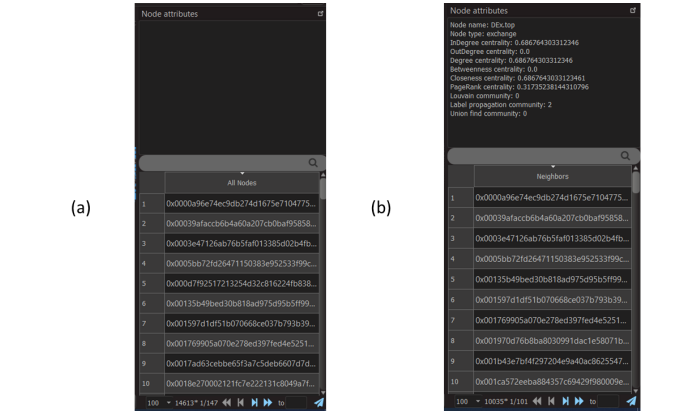
\includegraphics[width=\textwidth]{gfx/node-view.png}
\caption{Node view displays attribute values and names of nodes (a) before clicking a node and (b) after clicking a node.}
\label{fig:node-view}
\end{figure}

The node view is to list out the information of a clicked node. Before clicking a node (Fig. \ref{fig:node-view}a), the values of node attributes are blank, and a list of all nodes is shown below the node attributes. After clicking a node (Fig. \ref{fig:node-view}b), the values of node attributes are displayed, and its neighbor nodes are shown below the node attributes.

\subsection{Control View}
\label{sec:methodology:view:control}

\begin{figure}[htb]
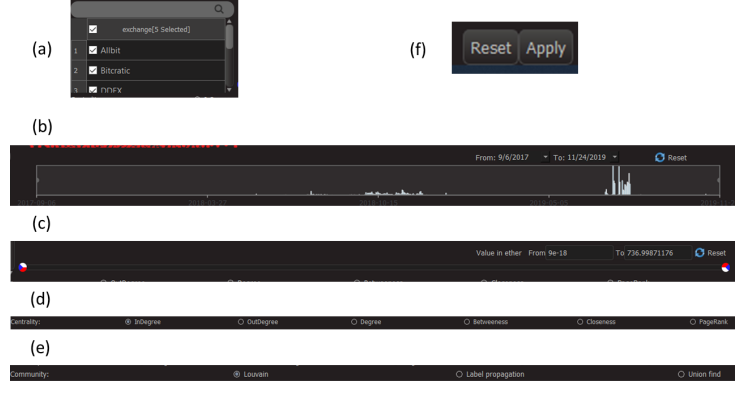
\includegraphics[width=\textwidth]{gfx/control-view.png}
\caption{Control view includes (a) options to filter the selected exchanges, (b) time brush to filter transactions within a specific period, (c) value slider to filter transactions within a specified range, (d) options to select a centrality measure, (e) options to select a community measure, and (f) "Reset" and "Apply" buttons.}
\label{fig:control-view}
\end{figure}

The control view contains filters of transactions for selected exchanges (Fig. \ref{fig:control-view}a), selected time interval (Fig. \ref{fig:control-view}b), and corresponding value range (Fig. \ref{fig:control-view}c), and selection options of centrality measure (Fig. \ref{fig:control-view}d) and community measure (Fig. \ref{fig:control-view}e). The "Reset" button sets the filters and selections to default values while the "Apply" button sets the filters and selections effective.

After filtering the transactions by exchange, a subgraph contains only those nodes and edges to represent the transactions with from address or to address as the specified exchanges.

After filtering the transactions by a time brush, a subgraph containing nodes and edges to represent transactions within the specified time interval is present. To observe the evolution of graph structure or the changes of graph over time, the time brush starts from a fixed time point, then it is moved at increments with the "Apply" button being pressed. As a result, the "growth" of graph can be revealed for evolution analysis.

After filtering the transactions by a value slider, the transactions within the specified value range are represented by a subgraph of nodes and edges, this value range refers to value in ether for MFG and number of calls for CIG and is not applicable for CCG. To observe the transactions at increasing weight, the value slider has a fixed end, then it is moved to right gradually with the "Apply" button taking effect. As a result, the graph with high edge weights "floats" on the surface.

The selection options for centrality measures consist of in-degree centrality, out-degree centrality, degree centrality, betweenness centrality, closeness centrality and PageRank centrality. The centrality value is positively correlated to the node size.

The selection options for community measures include Louvain community, label propagation community and union find community. The community cluster which a node is assigned to determines the node color.

% \section{Conclusion}
% \label{sec:system:conclusion}

% \blindtext
	% INCLUDE: methodology
% !TEX root = ../thesis.tex
%
\chapter{Applications}
\label{sec:applications}

% \cleanchapterquote{Users do not care about what is inside the box, as long as the box does what they need done.}{Jef Raskin}{about Human Computer Interfaces}

% \blindtext
% 4. Applications
% (i.e., What applications can benefit from your work. ) You could conduct several case studies to illustrate them. For example, graph analysis, evolutionary study, attack detection, etc. (Some could be found from the papers I sent you before) 

The approach of this thesis provides the macro view and micro view for the evolution of Ethereum transactions, it can identify overall trends as well as subset details of transactions for applications such as abnormality detection, impact analysis and evolutionary study.

\section{Abnormality Detection}
\label{sec:applications:abnormality}

% \blindtext
In the section \ref{sec:methodology:analysis:statistics}, the daily descriptive statistics over the entire period are computed to draw time plots. From the perspective of statistical analysis, the statistics should stay within certain number of standard deviations from their means for most of the time, otherwise they can be considered as abnormal.

The occurrence of abnormality can be the result reflecting existing events or the indication of future events, its detection assists us in identifying the existing events or predicting the future events.

From the macro view, this thesis monitors the daily numbers of created contracts, contract creators, refund records, refunders to detect abnormality in the growth of smart contracts.

\section{Impact Analysis}
\label{sec:applications:impact}

% \blindtext
There were certain significant events such as the launch of stable currency and cyber attack to steal cryptocurrency that cause positive or negative impact to the Ethereum blockchain. Compared with individual accounts, the exchanges can be stronger indicators to reflect the distribution of impact for these significant events. 

In the section \ref{sec:methodology:view}, the exchanges and activities can be selected by users to construct and visualize graphs over time. To assess the impact of a significant event on Ethereum exchanges, users can select the exchanges and activities covering the period before and after the occurrence of the event, and visualize the graphs during the period to observe the distribution of impact on different exchanges for different activities. 

\section{Evolutionary Study}
\label{sec:applications:evolutionary}

% \blindtext
It can be difficult to understand the evolution of individual accounts in terms of their importance and relationships with other accounts without transforming historical transaction data into graphs over time.

In the section \ref{sec:methodology:view}, centrality measures and community measures are computed for each account and they are represented by node sizes and node colors respectively for graph visualization. The program can project the growth of individual accounts by visualizing their history with dynamic graphs.

% 4. and the potential applications of the developed system."
\section{Machine Learning}
\label{sec:applications:learning}

% \blindtext
The data and algorithms are two core components of machine learning applications. For the data part, the training data and test data for pattern recognition of graph evolution is difficult to obtain. The fundamental problem is how to define the labels or clusters for certain patterns or groups, the program developed for graph visualization in this paper provides the first step to explore the graph patterns in Ethereum transactions.

From the above applications where decentralized exchanges are studied to observe the abnormal change in transaction activities, distribution of impact to different individual nodes, growth in importance and neighborhood relationships. All of them exhibit certain patterns, some of them may be regular patterns. If the research dataset is scaled up, different types of exchanges are included, or exchanges from different regions are included, or different categories of applications are included. An increasing amount of patterns are expected to be discovered, these can constitute the training dataset or test dataset if processed systematically.

% \section{Method}
% \label{sec:feature:theory}

% \blindtext

% \section{Experimental Results}
% \label{sec:feature:results}

% \blindtext

% \section{Summary}
% \label{sec:feature:summary}

% \blindtext
 % INCLUDE: applications
% !TEX root = ../thesis.tex
%
\chapter{Evaluation}
\label{sec:evaluation}

% \cleanchapterquote{Users do not care about what is inside the box, as long as the box does what they need done.}{Jef Raskin}{about Human Computer Interfaces}

% \blindtext
% 5. Evaluation 
% (Experimental results, (1) Visualization; (2) Performance; (3) Applications)

\section{Abnormality Detection}
\label{sec:evaluation:abnormality}

The growth of smart contracts is analyzed by two types of statistics namely creation statistics and decreation statistics. Creation statistics which are associated with positive growth of smart contracts include daily number of created contracts and contract creators. Decreation statistics which are associated with negative growth of smart contracts include daily number of refund records and refunders. These statistics are visualized with time plots to detect abnormal changes.

\subsection{Creation Statistics}
\label{sec:evaluation:abnormality:creation}

\begin{table}[h]
\caption{Daily number of created contracts}
\label{tab:created-contracts}
\renewcommand\arraystretch{0.7}
\begin{tabular}{@{}cc@{}}
\toprule
\multicolumn{2}{c}{Created Contracts} \\
\midrule
Average                & 12267.14442    \\
Standard Error         & 366.8075104    \\
Median                 & 7510.5         \\
Mode                   & 7267           \\
Standard Deviation     & 11089.48345    \\
Variance               & 122976643.2    \\
Kurtosis               & 2.305335977    \\
Skewness               & 1.789698857    \\
Minimum                & 650            \\
Maximum                & 52959          \\
Summation              & 11212170       \\
Observation            & 914            \\
\bottomrule
\end{tabular}
\end{table}

From the descriptive statistics of created contracts in 914 days in Table \ref{tab:created-contracts}, the daily numbers of created contracts ranging from 650 to 52959 had a mean at 12267 and a standard deviation at 11089, the high ratio of standard deviation to mean indicated a large variation in the distribution. With reference to a normal distribution which has skewness and relative kurtosis both at 0, skewness and kurtosis measure the deviation from normal distribution in terms of degree of asymmetry and portion of outliers respectively. The daily numbers of created contracts had skewness at 1.79 and kurtosis at 2.31, its distribution was right-skewed and had low portion of outliers.

\begin{figure}[htb]
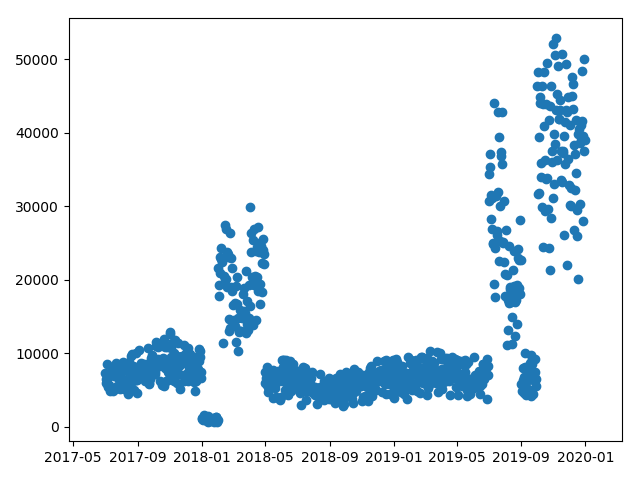
\includegraphics[width=0.7\textwidth]{gfx/created-contracts.png}
\caption{Daily number of created contracts}
\label{fig:created-contracts}
\end{figure}

From the time plot of created contracts in Fig. \ref{fig:created-contracts}, the daily numbers of created contracts had different activity levels in four time intervals. The first interval was before January 2018, the activity level was low with a flat trend. The second interval was from January to May 2018, the activity level rose sharply and reached a peak. The third interval is from June 2018 to June 2019, the activity level dropped sharply and remained a flat trend. The fourth interval was after June 2019, the activity level rose sharply and reached another peak.

\begin{table}[h]
\caption{Daily number of contract creators}
\label{tab:contract-creators}
\renewcommand\arraystretch{0.7}
\begin{tabular}{@{}cc@{}}
\toprule
\multicolumn{2}{c}{Contract Creators} \\
\midrule
Average            & 5343.724 \\
Standard   Error   & 100.7515 \\
Median             & 5278     \\
Mode               & 1474     \\
Standard Deviation & 3045.963 \\
Variance           & 9277890  \\
Kurtosis           & -1.05016 \\
Skewness           & 0.139566 \\
Range              & 12489    \\
Minimum            & 250      \\
Maximum            & 12739    \\
Summation          & 4884164  \\
Observation        & 914      \\
\bottomrule
\end{tabular}
\end{table}

From the descriptive statistics of contract creators in Table \ref{tab:contract-creators}, the daily numbers of contract creators ranging from 250 to 12739 had a mean at 5344 and a standard deviation at 3046, the high ratio of standard deviation to mean indicated a large variation in the distribution. The daily numbers of contract creators had skewness at 0.14 and kurtosis at -1.05, its distribution was slightly right-skewed and had moderately high portion of outliers.

\begin{figure}[htb]
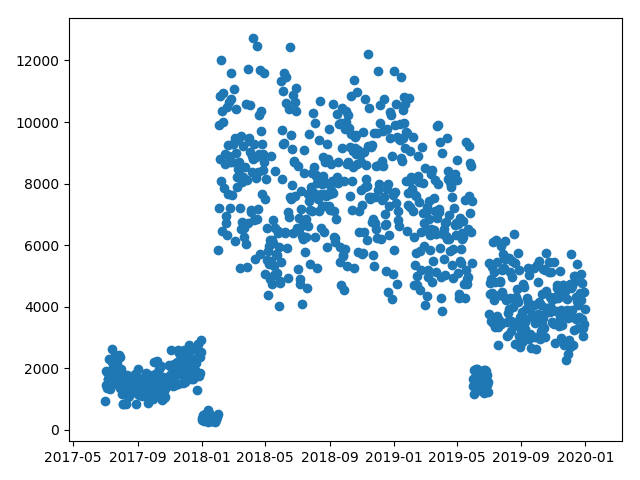
\includegraphics[width=0.7\textwidth]{gfx/contract-creators.png}
\caption{Daily number of contract creators}
\label{fig:contract-creators}
\end{figure}

From the time plot of contract creators in Fig. \ref{fig:contract-creators}, the daily numbers of contract creators had different activity levels in three time intervals. The first interval was before February 2018, the activity level was low with a flat trend. The second interval was from February 2018 to May 2019, the activity level reached a peak and fluctuated with direction. The third interval is after May 2019, the activity level dropped sharply and fluctuated without direction.

\subsection{Decreation Statistics}
\label{sec:evaluation:abnormality:decreation}

\begin{table}[h]
\caption{Daily number of refund records}
\label{tab:refund-records}
\renewcommand\arraystretch{0.7}
\begin{tabular}{@{}cc@{}}
\toprule
\multicolumn{2}{c}{Refund Records} \\
\midrule
Average                & 246067.8654    \\
Standard Error         & 9534.322429    \\
Median                 & 87599.5        \\
Mode                   & 67             \\
Standard   Deviation   & 288245.7632    \\
Variance               & 83085620024    \\
Kurtosis               & -0.193791222   \\
Skewness               & 0.953646715    \\
Range                  & 1093572        \\
Minimum                & 52             \\
Maximum                & 1093624        \\
Summation              & 224906029      \\
Observation            & 914            \\
\bottomrule
\end{tabular}
\end{table}

From the descriptive statistics of refund records in Table \ref{tab:refund-records}, the daily numbers of refund records ranging from 52 to 1093624 had a mean at 246068 and a standard deviation at 288246, the high ratio of standard deviation to mean indicated a large variation in the distribution. The daily numbers of refund records had skewness at 0.95 and kurtosis at -0.19, its distribution was moderately right-skewed and had slightly high portion of outliers.

\begin{figure}[htb]
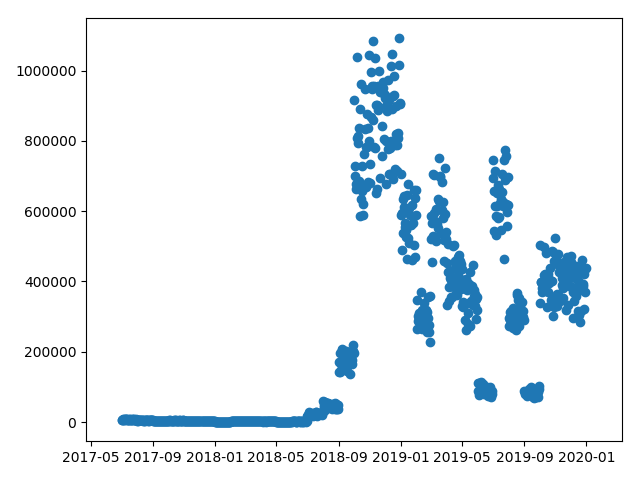
\includegraphics[width=0.7\textwidth]{gfx/refund-records.png}
\caption{Daily number of refund records}
\label{fig:refund-records}
\end{figure}

From the time plot of refund records in Fig. \ref{fig:refund-records}, the daily numbers of refund records had different activity levels in two time intervals. The first interval was before September 2018, the activity level was low with a flat trend. The second interval was after September 2018, the activity level reached a peak and fluctuated without direction.

\begin{table}[h]
\caption{Daily number of refunders}
\label{tab:refunders}
\renewcommand\arraystretch{0.7}
\begin{tabular}{@{}cc@{}}
\toprule
\multicolumn{2}{c}{Refunders} \\
\midrule
Average                       & 276.2144           \\
Standard Error                & 15.22506           \\
Median                        & 111                \\
Mode                          & 81                 \\
Standard Deviation            & 460.2905           \\
Variance                      & 211867.4           \\
Kurtosis                      & 15.55016           \\
Skewness                      & 3.759675           \\
Range                         & 3169               \\
Minimum                       & 5                  \\
Maximum                       & 3174               \\
Summation                     & 252460             \\
Observation                   & 914                \\
\bottomrule
\end{tabular}
\end{table}

From the descriptive statistics of refunders in Table \ref{tab:refunders}, the daily numbers of refunders ranging from 5 to 3174 had a mean at 276 and a standard deviation at 460, the high ratio of standard deviation to mean indicated a large variation in the distribution. The daily numbers of refunders had skewness at 3.76 and kurtosis at 15.55, its distribution was right-skewed and had low portion of outliers.

\begin{figure}[htb]
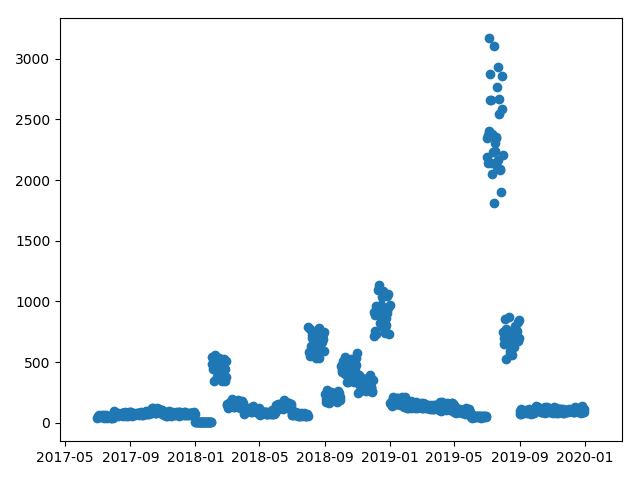
\includegraphics[width=0.7\textwidth]{gfx/refunders.png}
\caption{Daily number of refunders}
\label{fig:refunders}
\end{figure}

From the time plot of refunders in Fig. \ref{fig:refunders}, the daily numbers of refunders had different activity levels in three time intervals. The first interval was before July 2019, the activity level was low and flucuated without direction. The second interval was from July to September 2019, the activity level rose sharply and reached a peak. The third interval was after September 2019, the activity level dropped sharply and remained a flat trend.

\subsection{Significant Event}
\label{sec:evaluation:abnormality:event}

From the descriptive statistics of smart contract growth in section \ref{sec:evaluation:abnormality:creation} and section \ref{sec:evaluation:abnormality:decreation}, 2018 was a special year when abnormal changes in activity level took place. Around this year, there was a significant event in Ethereum blockchain, the issuance of a stable currency called Dai.

At the end of 2017, Dai built by Maker Foundation was issued as an ERC-20 token. Unlike Bitcoin which has volatile value and acts more like an investment than cash, Dai is marketed as a digital version of real money and its value consistently tracks the USD. To maintain stable value relative to USD, it is backed by assets which value is locked in publicly viewable smart contracts and adjusted automatically by algorithm. By removing the volatility of a typical cryptocurrency, Dai can store and exchange value like traditional money to serve many financial applications such as spending and lending, this can be a reason that activity level of smart contracts increased sharply for 2018.

\section{Impact Analysis}
\label{sec:evaluation:impact}

% \blindtext
In 2018 after the stable coin Dai was issued, the activities of exchanges including money transfer, smart contract creation, smart contract invocation could partially reflect the distribution of its impact. For example, the CIG representing contract invocation activities of decentralized exchanges can be further analyzed as decentralized exchanges had much less activities in money transfer and smart contract creation in 2018. To be clear, the exchanges are classified as decentralized exchanges in the exchange directory on EtherScan \cite{17}.

\begin{figure}[htb]
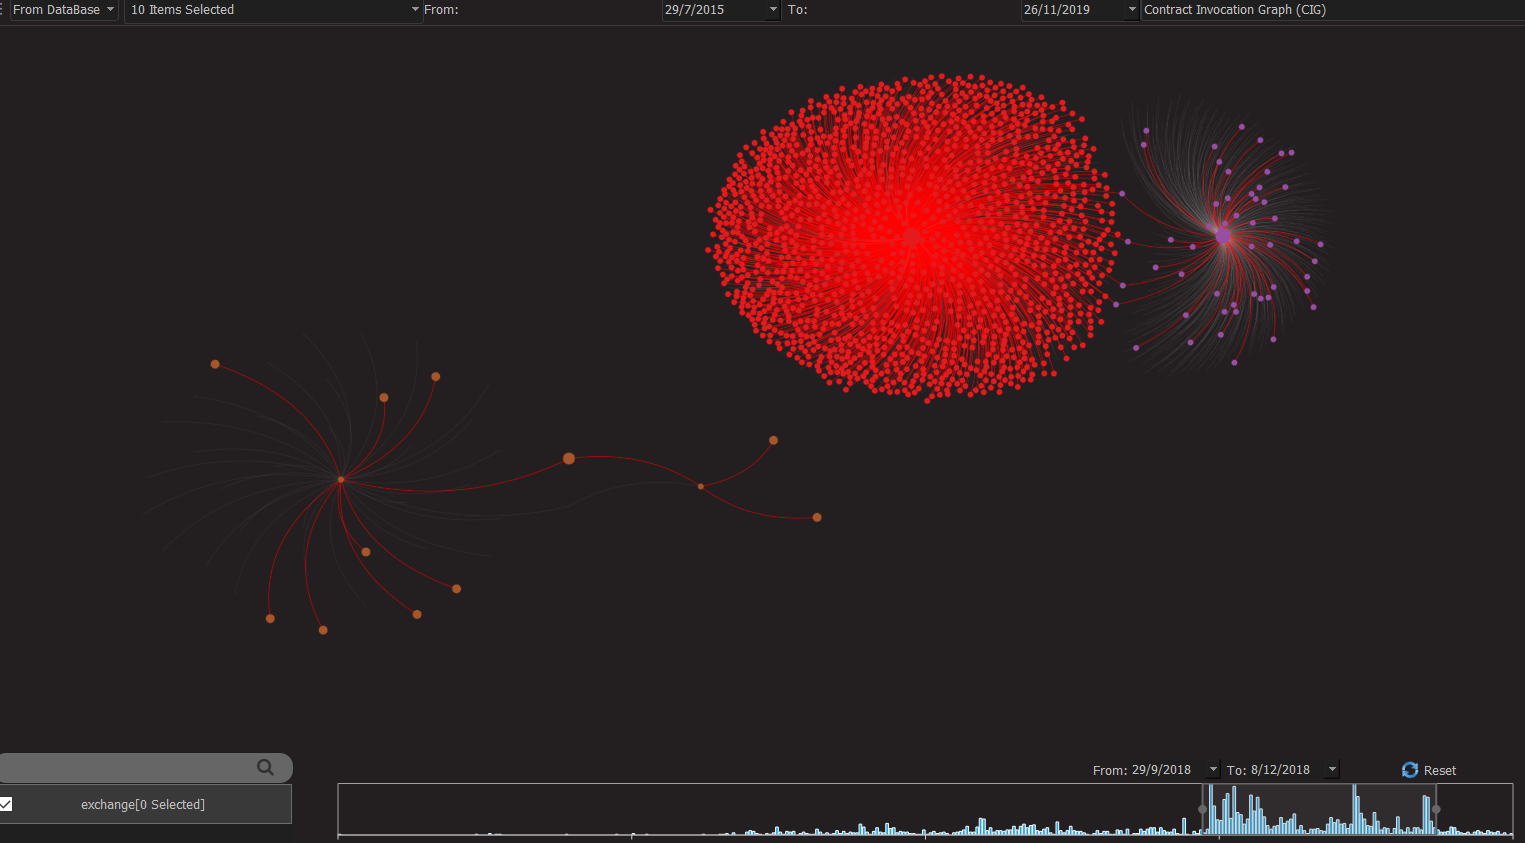
\includegraphics[width=\textwidth]{gfx/impact-analysis.png}
\caption{CIG of decentralized exchanges in selected interval}
\label{fig:impact-analysis}
\end{figure}

In the selected time interval covering highest activity levels in smart contract invocation by decentralized exchanges in 2018, Fig. \ref{fig:impact-analysis} illustrates the distribution of contribution to these activity levels for different exchanges. Among them, the decentralized exchange "Allbit" as a contract had most transactions associated with it. During this period from Oct 2018 to Dec 2018, "Allbit" introduced Dai coin into its products on 12 Oct \cite{22}. It was probably one of the reasons to attract high contract invocation activity in this period. 

\section{Evolutionary Study}
\label{sec:evaluation:evolution}

% \blindtext
One focus of evolutionary study is to analyze the growth of an individual in terms of its importance and relationships with other parties. In Fig. \ref{fig:impact-analysis} it shows that "Allbit" contributed the highest transaction volume in smart contract invocation among decentralized exchanges in 2018, it is worth noting that it was also launched in 2018. Therefore, the CIG in four incremental time intervals are visualized to analyze the changes of its importance and relationships with others.

\begin{figure}[htb]
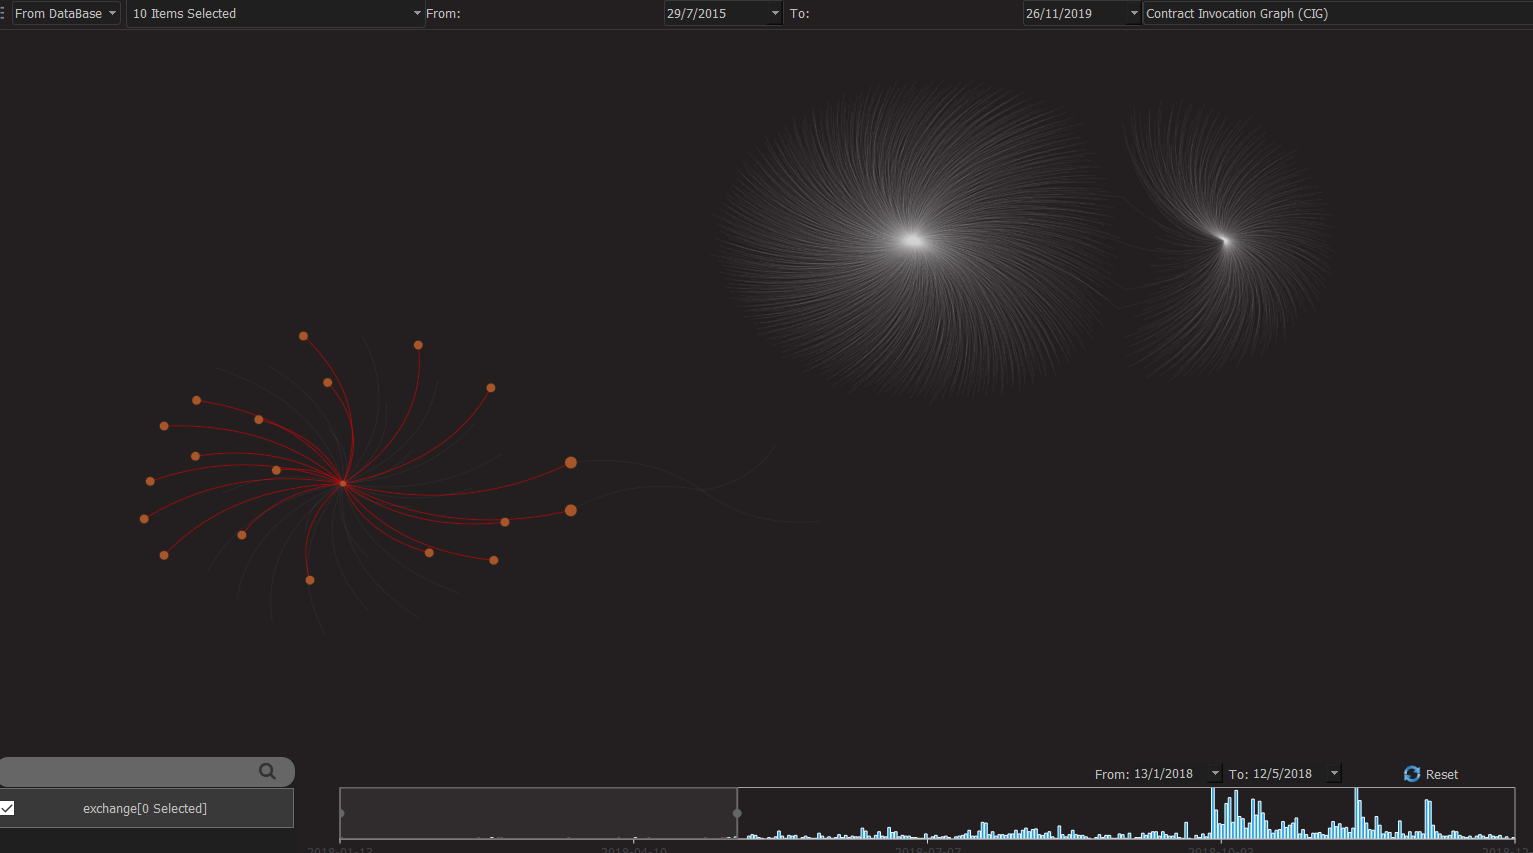
\includegraphics[width=0.7\textwidth]{gfx/evolutionary-study1.png}
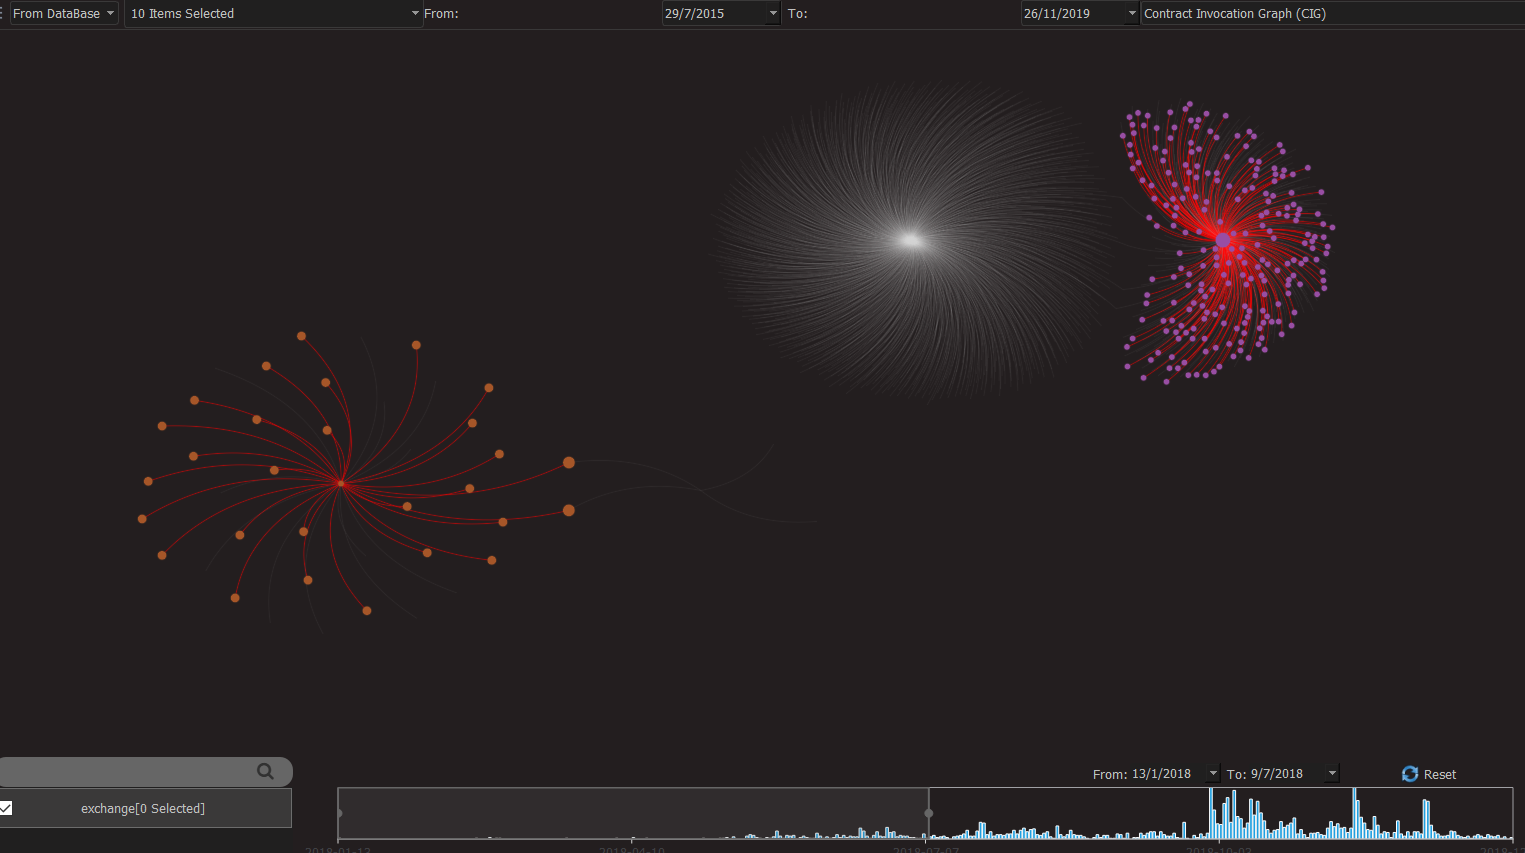
\includegraphics[width=0.7\textwidth]{gfx/evolutionary-study2.png}
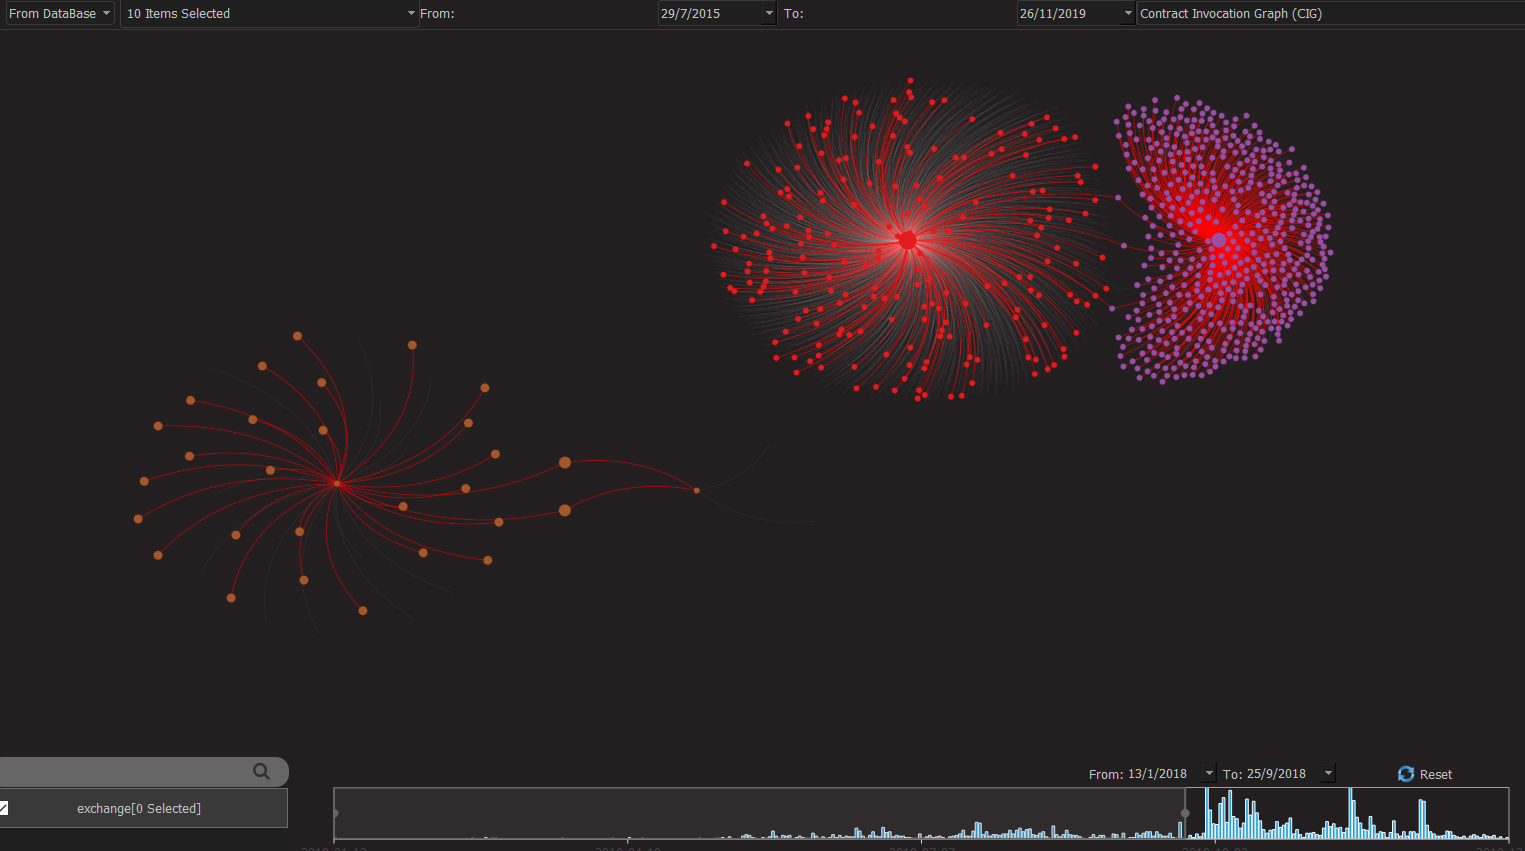
\includegraphics[width=0.7\textwidth]{gfx/evolutionary-study3.png}
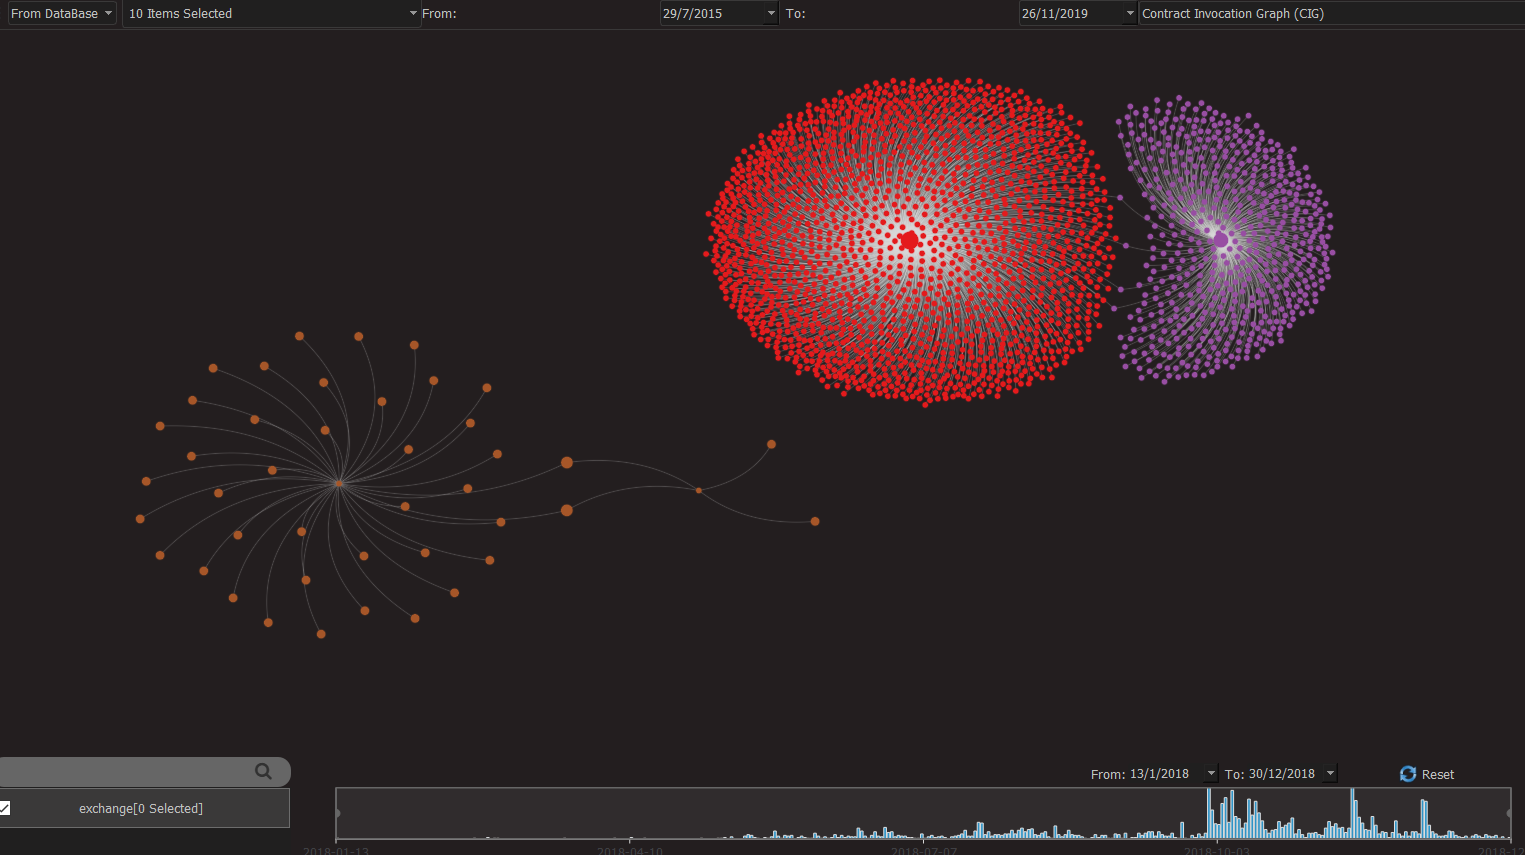
\includegraphics[width=0.7\textwidth]{gfx/evolutionary-study4.png}
\caption{CIG of decentralized exchanges in incremental intervals}
\label{fig:evolutionary-study}
\end{figure}

From Fig. \ref{fig:evolutionary-study}, "Allbit" gained the highest degree centrality and formed the largest Louvain community among decentralized exchanges in 2018. "Allbit" was launched after the launch of "DEx.top" when "DEx.top" had certain degree of market share at that moment, then "Allbit" grew at a much higher speed than "Dex.top", eventually "Allbit" exceeded its competitor "DEx.top" in centrality and community measures after adding Dai currency as its product. In Fig. \ref{fig:impact-analysis}, it can also be observed that when "Allbit" reached peak transaction volume, "DEx.top" only had little growth \cite{23}.


% \section{Summary}
% \label{sec:real:summary}

% \blindtext
 % INCLUDE: evaluation
% !TEX root = ../thesis.tex
%

\chapter{Conclusion}
\label{sec:conclusion}

% \blindtext
% 1. Macroview (All transactions without sampling, Daily transactions not entire period), 2. Microview (Specification of period and groups, Open-source and customizable program), 3. Improvements (More parallel computing, More precalculated data)

\section{Major Contributions}
\label{sec:conclusion:contributions}

% \blindtext
The aim of this thesis is to provide the approach and tools for analyzing the evolution of Ethereum transactions. The approach consists of macroview and microview supplemented with appropriate tools.

For the macroview, it covers all the Ethereum transactions from 30 Jul 2015 to 25 Nov 2019 without downsampling, and groups the transactions by day instead of the entire period to increase accuracy.

For the microview, it is visualized by an application developed in this thesis in the form of graphs over time, this application allows users to select accounts and time intervals which enable more flexible graph generation, it is open-source to non-developers for direct implementation or to developers for further customization.

\section{Future Improvements}
\label{sec:conclusion:improvements}

% \blindtext
Regarding the application program for graph visualization, its computing performance should be improved in the future to handle larger datasets in shorter time. For example, it can include more parallel computing and pre-calculated data.

For parallel computing, the independent components under computation are identified as much as possible, then they are processed concurrently by techniques such as MapReduce or matrix operation.

For pre-calculated data, it contains the smallest units which can be calculated independently, they remain relatively constant and are usually the results of repetitive calculations. They are identified as much as possible to reduce the time for repetitive calculations.

 % INCLUDE: conclusion
\cleardoublepage

% --------------------------
% Back matter
% --------------------------
{%
\setstretch{1.1}
\renewcommand{\bibfont}{\normalfont\small}
\setlength{\biblabelsep}{0pt}
\setlength{\bibitemsep}{0.5\baselineskip plus 0.5\baselineskip}
\nocite{*}
\printbibliography[title={References},nottype=online]
\printbibliography[heading=subbibliography,title={Websites},type=online,prefixnumbers={@}]
}
\cleardoublepage


% **************************************************
% End of Document CONTENT
% **************************************************
\end{document}
